\section{Über das Team}
\setauthor{Antonio Peric}
\begin{table}[h]
    \centering
    \caption{\textit{Tabelle 1.1: Informationen über den Bertreuer und Partner.}}
    \begin{tabular}{|p{0.5\textwidth}|p{0.5\textwidth}|}
        \hline
        Bertreuer & Prof. Mag. Ing. Hans Christian Hammer \\ \hline
        Partner & DI. Christian Aberger \\ \hline
    \end{tabular}
\end{table}

\section{Bertreuer und Partner}
\setauthor{Antonio Peric}
\begin{table}[h]
    \centering
    \caption{\textit{Tabelle 1.2: Informationen über das Projekt und das Team.}}
    \begin{tabular}{|p{0.5\textwidth}|p{0.5\textwidth}|}
        \hline
        Projektname & AGM - Abergymmobile \\ \hline
        Teamleiter & Antonio Kuvac \\ \hline
        Teammitglieder & Antonio Kuvac, Antonio Peric \\ \hline
        Erstellt am & 12.7.2023 \\ \hline
    \end{tabular}
\end{table}

\section{Ausgangssituation und Zielstellung}

\subsection{Ausgangssituation}
\setauthor{Antonio Peric}   
Aktuell ist der Prozess der Trainingsplangenerierung und -verwaltung im 
Fitnessstudio LionFit ineffizient und umständlich für Kunden*innen. 
Daher möchte das Fitnessstudio eine digitale Lösung implementieren,
um den Prozess zu vereinfachen und die Effizienz zu steigern. 
Derzeit werden die Trainingspläne in einer Web-Applikation 
erstellt und als PDF ausgedruckt, während die Trainingsdaten 
auf dem ausgedruckten PDF erfasst werden. Dieser Prozess ist 
unpraktisch, da die Kunden*innen bei jeder Trainingseinheit ein 
ausgedrucktes PDF mitnehmen und die Daten manuell eingeben müssen.

\subsection{Zieldefinition}
\setauthor{Antonio Peric}  
Die Entwicklung einer nativen App für Android-Geräte zur Umsetzung von Trainingsplänen in einem Fitnessstudio gewinnt zunehmend an Bedeutung. Diese App ermöglicht es den Nutzer*innen, ihre individuellen Trainingspläne effektiv und effizient abzuarbeiten, 
\newline
\newline
Die Trainingsplanverwaltung stellt sicher, dass die Daten des Trainingsplans aktuell und auf die Bedürfnisse der*die Nutzer*innen zugeschnitten sind. Durch die Anbindung der App an die Trainingsplanverwaltung wird es ermöglicht, die relevanten Daten direkt auf dem Android-Gerät der*die Nutzer*innen abzurufen. Dies erleichtert die Organisation und Durchführung des Trainings, indem es den Nutzer*innen erlaubt, auf ihre individuellen Trainingspläne in Echtzeit zuzugreifen.
\newline
\newline
Am Ende einer Trainingssession werden die Trainingsdaten, wie beispielsweise die Anzahl der Wiederholungen, die Gewichte oder die Trainingsdauer, in die Trainingsdatenbank übertragen und gespeichert. Dies ermöglicht eine kontinuierliche Analyse und Anpassung der Trainingspläne, um eine optimale Unterstützung der*die Nutzer*innen in ihrer sportlichen Entwicklung zu gewährleisten.
\newline
\newline
Durch die Integration von Training und Datenverwaltung in einer nativen Android-App werden Fitnessstudios in die Lage versetzt, ein benutzerfreundliches, modernes und zielgerichtetes Trainingsumfeld für ihre Mitglieder*innen zu schaffen. Das trägt zur Steigerung der Motivation und der Erfolgschancen bei, da individuelle Trainingsziele leichter erreicht werden können.

\newpage
\subsection{Nicht Ziele}
\setauthor{Antonio Peric}  
Die Entwicklung einer App für Trainingspläne in Fitnessstudios birgt auch gewisse Herausforderungen und Risiken. Eine davon ist die Gefahr, eine zu komplex gestaltete App zu entwickeln, die den Nutzer*innen Schwierigkeiten bereitet und sie dazu veranlasst, stattdessen auf den traditionellen Zettel-Trainingsplan zurückzugreifen. Um dem entgegenzuwirken, sollte die App intuitiv und benutzerfreundlich gestaltet sein, sodass sie die Bedürfnisse der*die Nutzer*innen erfüllt und gleichzeitig den Trainingsprozess vereinfacht.
\newline
\newline
Ein weiteres Risiko besteht in der Entwicklung einer fehlerhaften App, die den Nutzer*innen Unannehmlichkeiten bereitet und ihre Trainingserfahrung beeinträchtigt. Um dies zu vermeiden, ist es wichtig, die App sorgfältig zu testen und mögliche Fehlerquellen frühzeitig zu identifizieren. Die Qualitätssicherung und regelmäßige Aktualisierung der App sind entscheidend für ihren Erfolg.
\newline
\newline
Schließlich kann auch das Design der App einen bedeutenden Einfluss auf die Akzeptanz bei den Nutzer*innen haben. Eine App, deren Design die Zielgruppe nicht anspricht, könnte weniger erfolgreich sein und das Potenzial der digitalen Trainingsplanunterstützung ungenutzt lassen. Daher ist es ratsam, bei der Gestaltung der App auf ansprechende und funktionale Designelemente zu achten, die die Nutzer*innen ansprechen und zum wiederholten Gebrauch motivieren.
\newline
\newline
Die Berücksichtigung dieser Herausforderungen bei der Entwicklung einer Trainingsplan-App ist essentiell, um eine positive Benutzererfahrung zu gewährleisten und den Nutzer*innen eine effektive und ansprechende Alternative zum traditionellen Zettel-Trainingsplan zu bieten.

\newpage
\section{Zielgruppe}
\setauthor{Antonio Peric}  
Diese Zielgruppe umfasst sowohl regelmäßige Fitnessstudio-Besucher*innen als auch Sportler*innen, 
die unabhängig von einem Fitnessstudio trainieren und eine digitale Lösung für die Verwaltung 
ihrer Trainingspläne suchen. Besonders praktisch für diese Zielgruppe ist, dass sie jederzeit 
Zugang zu ihren Trainingsplänen und -daten auf ihrem Smartphone haben. Dies bietet mehr Flexibilität 
und Übersicht bei der Gestaltung und Überwachung des Trainings. Außerdem müssen die Kunden*innen nicht mehr 
auf ausgedruckte Trainingspläne zurückgreifen und können stattdessen auf eine sichere und zuverlässige 
digitale Lösung setzen.

\section{Funktionale Anforderungen}
\setauthor{Antonio Peric}  
Die Benutzeroberfläche der native App soll eine einfache und 
ansprechende Gestaltung aufweisen, um auch nicht computeraffinen Personen eine leichte 
Handhabung zu ermöglichen. Zusätzlich soll durch die Modernisierung des Trainingsplanprozesses 
die Kommunikation zwischen Verwaltung und Koordinatoren im Fitnessstudio LionFit vereinfacht 
und automatisiert werden.

\subsection{An die App}
\setauthor{Antonio Peric}  
Die effektive Nutzung einer Trainingsplan-App erfordert eine sorgfältige Planung und Umsetzung verschiedener Funktionen. Eine Möglichkeit, die Nutzer*innen in ihrem Trainingsprozess zu unterstützen, besteht darin, die Durcharbeitung der Trainingspläne als To-Do-Liste zu gestalten. Dies ermöglicht es den Nutzer*innen, ihre Fortschritte während des Trainings klar zu erkennen und ihre Motivation aufrechtzuerhalten.
\newline
\newline
Nach Abschluss jeder Übung sollte die App die Möglichkeit bieten, den Trainingsplan zu überprüfen und gegebenenfalls anzupassen. Dies ermöglicht eine individuelle Anpassung des Trainings und stellt sicher, dass die Nutzer*innen stets auf dem aktuellen Stand ihrer Trainingsziele sind. Die flexible Anpassung des Trainingsplans trägt dazu bei, die Effektivität des Trainings zu erhöhen und den Bedürfnissen der*die Nutzer*innen gerecht zu werden.
\newpage
Die Verfügbarkeit des überarbeiteten Trainingsplans zu jeder Zeit ist ein weiterer wichtiger Aspekt, der es den Nutzer*innen ermöglicht, ihre Trainingspläne erneut durchzuarbeiten und an ihren Zielen kontinuierlich zu arbeiten. Durch die ständige Verfügbarkeit der aktualisierten Trainingspläne können die Nutzer*innen ihre Trainingsfortschritte effizient verfolgen und die erforderlichen Anpassungen vornehmen.
\newline
\newline
Schließlich sollte die App auch eine Historie der alten Trainingspläne aufbewahren, um den Nutzer*innen einen Überblick über ihre Trainingsentwicklung und die Möglichkeit, auf vergangene Trainingspläne für zukünftige Referenzen zuzugreifen, zu bieten. Dies kann als wertvolles Instrument für die Selbstreflexion und Analyse des Trainingsfortschritts dienen.

\section{App}
\subsection{Allgemeine Beschreibung}
\setauthor{Antonio Peric}  
Mit unserer innovativen mobilen Anwendung bieten wir Ihnen die Möglichkeit, Ihre individuellen Trainingspläne bequem und effizient über Ihr Smartphone abzuarbeiten. Die Anwendung präsentiert den Nutzer*innen die Trainingspläne in Form einer leicht verständlichen To-Do-Liste, die eine strukturierte und systematische Durchführung jeder Übung gewährleistet. Dies fördert die Trainingsdisziplin und unterstützt die Nutzer*innen dabei, ihre persönlichen Trainingsziele zu erreichen.
\newline
\newline
Nach Abschluss jeder Übung haben die Nutzer*innen die Möglichkeit, ihren Trainingsplan zu überprüfen und gegebenenfalls anzupassen. Diese Flexibilität ermöglicht es, das Training kontinuierlich an die individuellen Bedürfnisse und Fortschritte der*die Nutzer*innen anzupassen, um eine optimale Trainingsgestaltung sicherzustellen.
\newline
\newline
Der überarbeitete Trainingsplan ist jederzeit für die Nutzer*innen zugänglich, sodass sie ihn bei Bedarf erneut durcharbeiten können. Dies gewährleistet eine hohe Verfügbarkeit der Trainingsinformationen und erleichtert die Planung und Durchführung des Trainings im Alltag der*die Nutzer*innen.
\newpage
Darüber hinaus werden alte Trainingspläne in der Anwendungshistorie gespeichert, sodass sie bei Bedarf als Referenz herangezogen werden können. Die Archivierung der Trainingshistorie ermöglicht den Nutzer*innen, ihren Trainingsfortschritt im Laufe der Zeit zu analysieren und eventuelle Anpassungen oder Modifikationen ihrer Trainingsziele vorzunehmen.

\subsection{Mockups}
\setauthor{Antonio Peric}  
Im Rahmen des Entwicklungsprozesses unserer mobilen Anwendung haben wir vier verschiedene Mockups erstellt, um das beste Design für die Nutzer*innen zu ermitteln und es optimal an die Bedürfnisse verschiedener Zielgruppen anzupassen. Die Gestaltung dieser Mockups berücksichtigt sowohl ästhetische als auch funktionale Aspekte, um eine ansprechende und effiziente Benutzeroberfläche zu schaffen, die den unterschiedlichen Anforderungen der*die Nutzer*innen gerecht wird.
\newline
\newline
Die vier Mockups wurden sorgfältig entworfen und auf Basis von Designprinzipien und Benutzeranforderungen entwickelt, um sicherzustellen, dass sie alle relevanten Funktionen und Interaktionen der Anwendung abbilden. Dabei wurde darauf geachtet, unterschiedliche Designansätze und Interaktionsmöglichkeiten zu berücksichtigen, um ein breites Spektrum an Nutzerpräferenzen abzudecken.
\newline
\newline
Nach einer umfassenden Analyse und Bewertung der vier Mockups haben unser Berater und Partner das vierte Mockup als das am besten geeignete Design ausgewählt. Dieses Design wurde aufgrund seiner benutzerfreundlichen Gestaltung, der klaren Struktur und der ansprechenden visuellen Elemente bevorzugt. Zudem wurde es als am ehesten in der Lage erachtet, die Bedürfnisse und Anforderungen der verschiedenen Zielgruppen zu erfüllen.

\newpage
Beim Öffnen der mobilen Anwendung gelangen die Nutzer*innen zunächst in den Log-in-Bereich (\hyperref[fig:log1]{siehe Abbildung 1}, \hyperref[fig:log2]{siehe Abbildung 2}). Hier besteht die Möglichkeit, sich mithilfe eines QR-Codes oder NFC-Technologie schnell und unkompliziert einzuloggen. Durch die Integration dieser modernen und benutzerfreundlichen Authentifizierungsmethoden wird der Zugang zur Anwendung für die Nutzer*innen erleichtert und die Sicherheit der persönlichen Daten gewährleistet.

\begin{figure}[!htb]
    \centering
    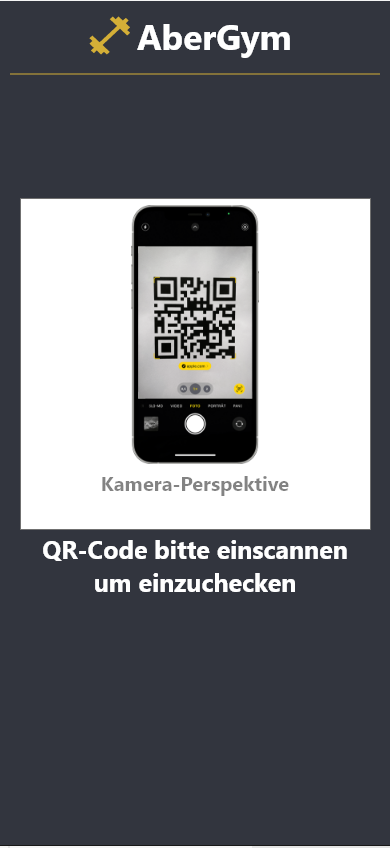
\includegraphics[width=0.35\textwidth]{pics/log1.png}
    \caption{Mockup 1 | Log-in-Bereich der mobilen Anwendung}
    \label{fig:log1}
\end{figure}
\begin{figure}[!htb]
    \centering
    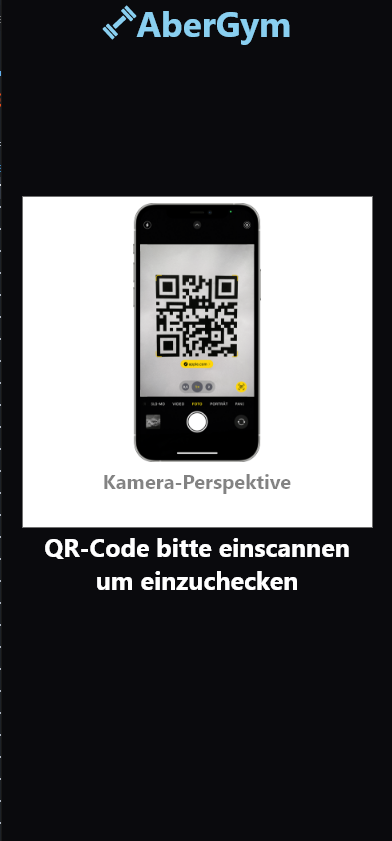
\includegraphics[width=0.35\textwidth]{pics/log2.png}
    \caption{Mockup 2 | Log-in-Bereich der mobilen Anwendung}
    \label{fig:log2}
\end{figure}
\FloatBarrier

Nach erfolgreichem Einloggen in die mobile Anwendung werden die Nutzer*innen automatisch zum heutigen Trainingsplan weitergeleitet. Dort besteht die Möglichkeit, den Trainingsplan jederzeit durch Berührung der Touchfläche {``Trainingsplan starten''} zu starten. Diese benutzerfreundliche Gestaltung ermöglicht einen schnellen Zugriff auf die wichtigsten Funktionen und erleichtert den Einstieg in das Training.
\newline
\newline
In der unteren Leiste, die in \hyperref[fig:main3]{Abbildung 3} und \hyperref[fig:main4]{siehe Abbildung 4} dargestellt ist, können die Nutzer*innen bequem zwischen dem letzten und dem heutigen Trainingsplan navigieren. Diese Funktion erleichtert den Zugriff auf vergangene und aktuelle Trainingspläne und bietet den Nutzer*innen eine flexible Möglichkeit, ihre Trainingshistorie und Fortschritte einzusehen und zu verwalten.

\begin{figure}[!htb]
    \centering
    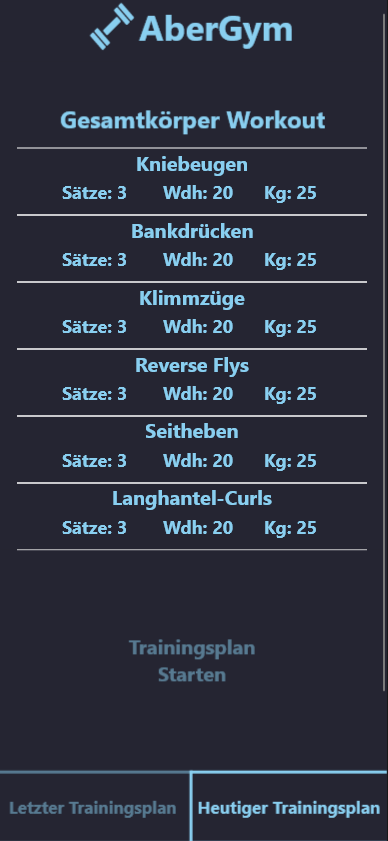
\includegraphics[width=0.35\textwidth]{pics/main3.png}
    \caption{Mockup 3 | Hauptbereich der mobilen Anwendung}
    \label{fig:main3}
\end{figure}
\begin{figure}[!htb]
    \centering
    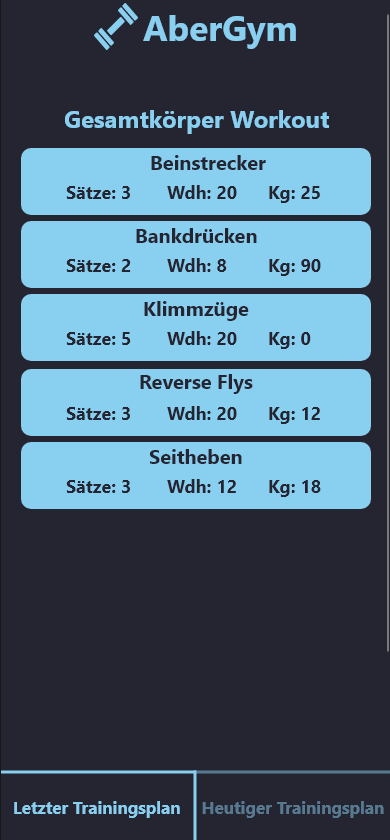
\includegraphics[width=0.35\textwidth]{pics/main4.png}
    \caption{Mockup 4 | Hauptbereich der mobilen Anwendung}
    \label{fig:main4}
\end{figure}
\FloatBarrier

Sobald die Nutzer*innen die Touchfläche {``Trainingsplan starten''} betätigen, wird der heutige Trainingsplan auf einer neuen Seite geöffnet und in einer To-Do-Ansicht präsentiert. In dieser Ansicht können die Nutzer*innen eine beliebige Übung auswählen und durchgehen. Zudem besteht die Möglichkeit, eine Übung zu bearbeiten, indem die Nutzer*innen die gewünschte Übung längere Zeit gedrückt halten. Diese flexible und benutzerfreundliche Gestaltung ermöglicht es den Nutzer*innen, ihren Trainingsplan individuell anzupassen und effizient durchzuarbeiten (\hyperref[fig:todolist1]{siehe Abbildung 5}, \hyperref[fig:todolist2]{siehe Abbildung 6}, \hyperref[fig:todolist3]{siehe Abbildung 7}, \hyperref[fig:todolist4]{siehe Abbildung 8}).

\begin{figure}[!htb]
    \centering
    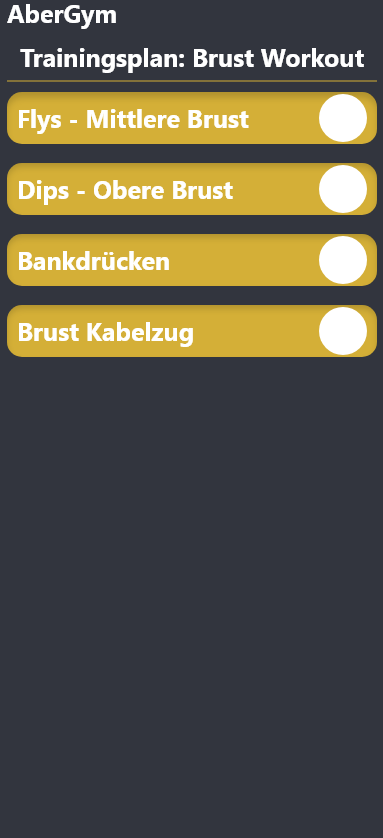
\includegraphics[width=0.35\textwidth]{pics/todolist1.png}
    \caption{Mockup 1 | To-Do-Bereich der mobilen Anwendung}
    \label{fig:todolist1}
\end{figure}
\begin{figure}[!htb]
    \centering
    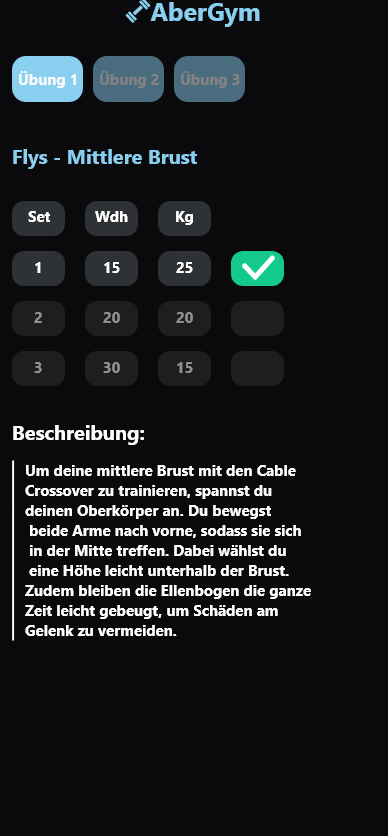
\includegraphics[width=0.35\textwidth]{pics/todolist2.png}
    \caption{Mockup 2 | To-Do-Bereich der mobilen Anwendung}
    \label{fig:todolist2}
\end{figure}
\begin{figure}[!htb]
    \centering
    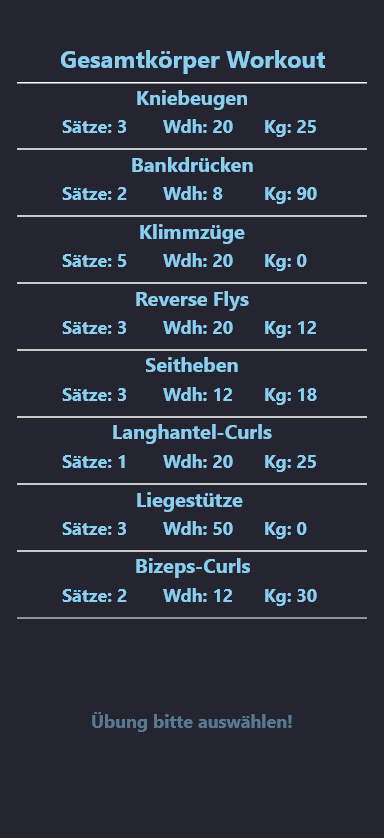
\includegraphics[width=0.35\textwidth]{pics/todolist3.png}
    \caption{Mockup 3 | To-Do-Bereich der mobilen Anwendung}
    \label{fig:todolist3}
\end{figure}
\begin{figure}[!htb]
    \centering
    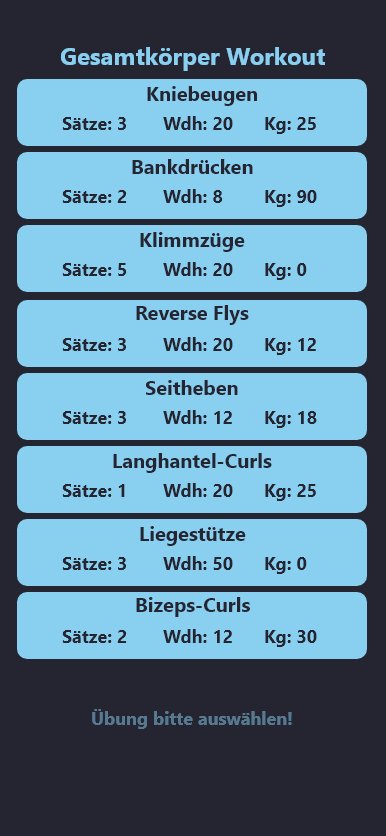
\includegraphics[width=0.35\textwidth]{pics/todolist4.png}
    \caption{Mockup 4 | To-Do-Bereich der mobilen Anwendung}
    \label{fig:todolist4}
\end{figure}
\FloatBarrier

Wenn die Nutzer*innen eine Übung auswählen, wird die entsprechende Übungsinformation erneut angezeigt. In jedem Mockup ist ein Zähler integriert, der bei Berührung des Bildschirms erhöht wird. Der gesamte Bildschirm dient als Druckfläche, um die Bedienung auch für Nutzer*innen mit Handschuhen zu erleichtern, da das Drücken von kleinen Buttons in solchen Situationen schwierig sein kann.
\newline
\newline
Sobald der Zähler den gleichen Wert wie die Satzanzahl der Übung erreicht hat, werden die Nutzer*innen automatisch zur To-Do-Ansicht zurückgeleitet. Die abgeschlossene Übung wird dann grau markiert und ans Ende der Liste verschoben. Dieses intuitive Design ermöglicht es den Nutzer*innen, ihren Fortschritt im Trainingsplan einfach nachzuvollziehen und sich auf die verbleibenden Übungen zu konzentrieren (\hyperref[fig:count1]{siehe Abbildung 9}, \hyperref[fig:todolist2]{siehe Abbildung 6}, \hyperref[fig:count3]{siehe Abbildung 11}, \hyperref[fig:count4]{siehe Abbildung 12}).

\begin{figure}[!htb]
    \centering
    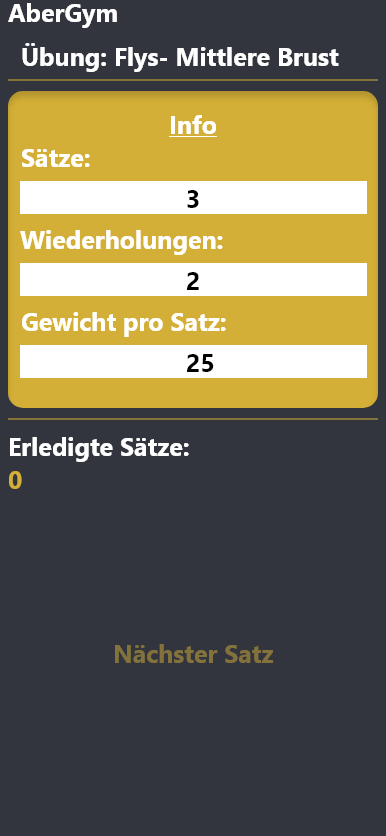
\includegraphics[width=0.35\textwidth]{pics/count1.png}
    \caption{Mockup 1 | Zähl-Bereich der mobilen Anwendung}
    \label{fig:count1}
\end{figure}
\begin{figure}[!htb]
    \centering
    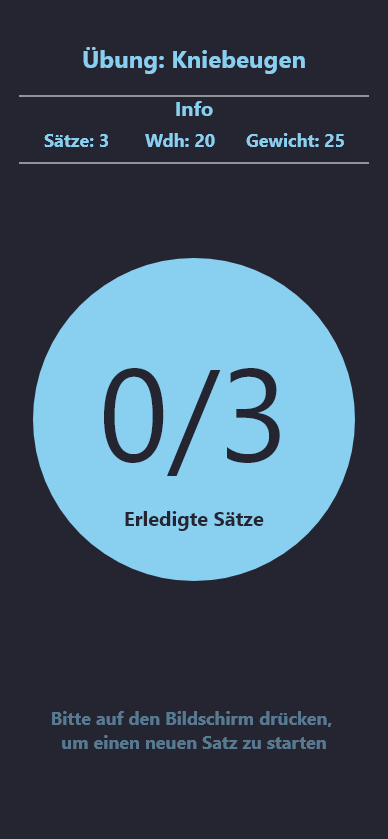
\includegraphics[width=0.35\textwidth]{pics/count3.png}
    \caption{Mockup 3 | Zähl-Bereich der mobilen Anwendung}
    \label{fig:count3}
\end{figure}
\begin{figure}[!htb]
    \centering
    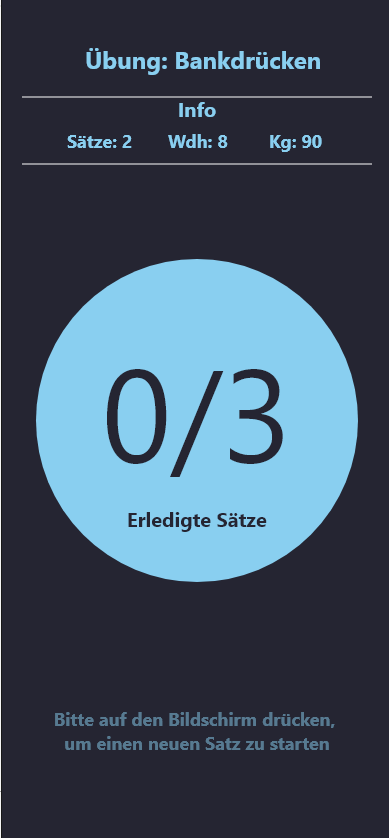
\includegraphics[width=0.35\textwidth]{pics/count4.png}
    \caption{Mockup 4 | Zähl-Bereich der mobilen Anwendung}
    \label{fig:count4}
\end{figure}
\FloatBarrier

Sobald die Nutzer*innen alle Übungen abgeschlossen haben, werden sie zur Hauptseite zurückgeleitet, auf der sie die vorgenommenen Änderungen während der Durchführung des Trainingsplans einsehen können. Der aktualisierte Trainingsplan, der die neuen Werte der jeweils bearbeiteten Übungen enthält, wird unter der Navigation "Heutiger Trainingsplan" angezeigt. Die Nutze*rinnen können den überarbeiteten Trainingsplan erneut durcharbeiten, indem sie die Touchfläche {``Trainingsplan starten''} betätigen.
\newline
\newline
In der Navigation "Letzter Trainingsplan" wird hingegen der ursprüngliche Trainingsplan mit den alten Daten der jeweiligen bearbeiteten Übungen dargestellt. Dieser kann jedoch nicht erneut gestartet werden. Diese Funktion ermöglicht den Nutzer*innen, die Fortschritte und Veränderungen im Trainingsplan nachzuvollziehen und die Entwicklung ihrer Trainingsergebnisse im Zeitverlauf zu verfolgen (\hyperref[fig:finished3]{siehe Abbildung 13}, \hyperref[fig:finished4]{siehe Abbildung 14}).

\begin{figure}[!htb]
    \centering
    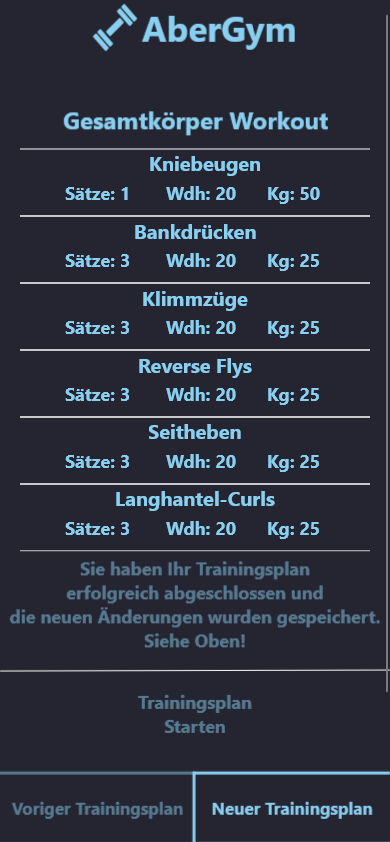
\includegraphics[width=0.35\textwidth]{pics/finished3.png}
    \caption{Mockup 3 | Hauptbereich nach der Durcharbeitung des Trainingplans}
    \label{fig:finished3}
\end{figure}
\begin{figure}[!htb]
    \centering
    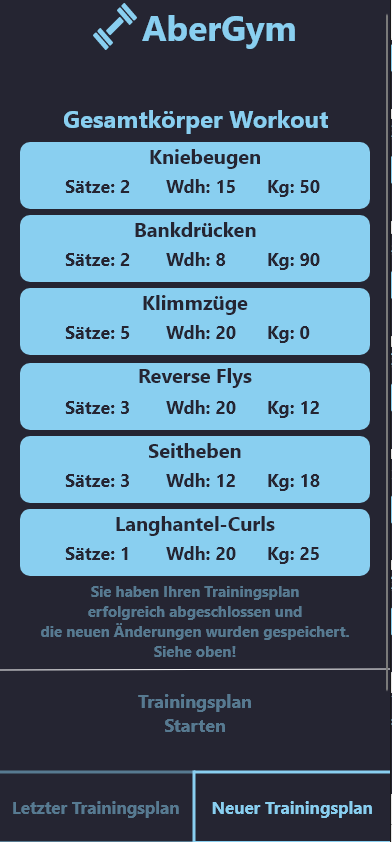
\includegraphics[width=0.35\textwidth]{pics/finished4.png}
    \caption{Mockup 4 | Hauptbereich nach der Durcharbeitung des Trainingplans}
    \label{fig:finished4}
\end{figure}
\FloatBarrier

Obwohl das Mockup 4 ursprünglich ausgewählt wurde, wurde während des Entwicklungsprozesses das Design weiter angepasst, optimiert und verschönert. Diese Änderungen wurden vorgenommen, um den Nutzer*innen die Navigation innerhalb der App zu erleichtern und ihnen dabei zu helfen, sich besser zurechtzufinden. Durch diese Designanpassungen wurde eine benutzerfreundliche und ansprechende Oberfläche geschaffen, die den Bedürfnissen und Erwartungen der-die Nutzer-innen entspricht.